\documentclass{standalone}
%
\usepackage{tikz}
\usetikzlibrary{backgrounds}
\usetikzlibrary{calc}
\usetikzlibrary{decorations.pathmorphing}
\usetikzlibrary{bending,arrows.meta}
\usetikzlibrary{shapes.callouts}
\usetikzlibrary{shapes.geometric}
\usetikzlibrary{shapes.arrows}
\usepackage{array}
%
\tikzstyle directed=[postaction={decorate,decoration={markings, mark=at position .5 with {\arrow{>}}}}]
%
\usepackage{tkz-euclide}
%
%\usepackage{dsfont}
%
\usepackage{xcolor}
\definecolor{space}{HTML}{1F2C4E}
\definecolor{earth}{HTML}{0089FA}
\definecolor{mars}{HTML}{DC7B4E}
\definecolor{dida}{HTML}{FFDE00}
\definecolor{title}{HTML}{FBA706}
\definecolor{linem}{HTML}{DBDBDB}
\definecolor{moon}{HTML}{AFAFAF}
\definecolor{craterm}{HTML}{616060}
\definecolor{core2}{HTML}{FF9616}
%
\usepackage{amsmath}
%
\usepackage{fontspec}
\setmainfont{Open Dyslexic}
%
\title{Viaggiatori nello spazio}
%
\begin{document}
	\tikzset{partial ellipse/.style args = {#1:#2:#3}{insert path={+ (#1:#3) arc (#1:#2:#3)}},
		notice/.style  = { draw, ellipse callout, callout relative pointer={#1} },
	}
	\begin{tikzpicture}[background rectangle/.style={fill=white},show background rectangle,>={[inset=0,angle'=27]Stealth},my arrow/.style={decorate,decoration={markings,mark=at position 0.5 with {\arrow[scale=1.5]{>}};}}]
		%title
		\draw [black,ultra thick,fill=title] (0,2) rectangle (30,-2);
		\node (example-textwidth-2) [right, align=center, text width=30cm, color=black, font=\fontsize{65pt}{66pt}\selectfont] at (0,0) {Viaggiatori nello spazio};
		%
		\begin{scope}[shift={(0,-15)}]
			% voyager
			\begin{scope}[shift={(5,0)},scale=0.8]
				\begin{scope}[rotate around={-100:(0,0)}]
					\begin{scope}[rotate around={20:(0,0)}]
						\draw [fill=linem] (0,0) -- (25,0) -- (25,0.5) -- (0,0.5) -- (0,0);
					\end{scope}
					\draw [fill=linem] (0,0) -- (-14.5,0) -- (-14.5,-1) -- (-15,-1) -- (-15.5,-1) -- (-15.5,0.5) -- (0,0.5) -- (0,0);
					
					\draw [fill=linem] (-3.5,1) -- (-2,-0.5) -- (2,-0.5) -- (3.5,1) -- (-3.5,1);
					\draw [fill=craterm] (0,0) circle (0.2 cm);
					\draw [fill=moon] (0,4.5) [partial ellipse=180:360:7.5 and 4];
					\draw [fill=linem](0,4.5) [partial ellipse=0:360:7.5 and 1];
					\draw [fill=craterm] (0,3.5) [partial ellipse=0:180:0.5 and 0.2];
					\draw [color=moon, line width=0.2 cm] (-4.5,4) -- (-0.4,9);
					\draw [color=moon, line width=0.2 cm] (4.5,4) -- (0.4,9);
					%
					\draw [fill=craterm] (0,9) [partial ellipse=180:360:0.5 and 0.2] -- (0.5,9) -- (0.5,10.5) -- (-0.5,10.5) -- (-0.5,9);
					\draw [fill=craterm] (0,10.5) [partial ellipse=0:360:0.5 and 0.2];
				\end{scope}
			\end{scope}
		\end{scope}
		% voyagers trajectories
		\begin{scope}[shift={(0,-67)}]
			\draw[fill=space] (0.5,5.5) rectangle (15,-5.5);
			\filldraw[white] (6,0) circle (0.1);
			\draw[color=white,ultra thick] (6,0) circle (0.2);
			\draw[color=white,ultra thick] (6,0) circle (0.9);
			\draw[color=white,ultra thick] (6,0) circle (1.6);
			\draw[color=white,ultra thick] (6,0) circle (3.1);
			\draw[color=white,ultra thick] (6,0) circle (5);
			\begin{scope}
				\draw[color=earth!50!white,ultra thick,directed,dashed] (6,0.2) arc[start angle=90, end angle=180,radius=0.5] -- (5.5,-0.3) arc[start angle=170, end angle=270,radius=1] -- (6.5,-1.45) arc[start angle=-86, end angle=-55,radius=5] -- (9,-0.55) arc[start angle=-60, end angle=-20,radius=5.2];
				\draw[color=red!50!mars,ultra thick,directed,dashed] (6,0.2) arc[start angle=70, end angle=180,radius=0.5] -- (5.31,-0.35) arc[start angle=165, end angle=260,radius=1] -- (6.15,-1.6) arc[start angle=-116, end angle=-85,radius=10];				
			\end{scope}
			\draw[fill=dida] (0.8,4.8) rectangle (12,6.2);
			\node (example-textwidth-2) [right, align=left, text width=11cm, color=black, font=\fontsize{14pt}{15pt}\selectfont] at (1,5.5) {Schema (non esatto) delle traiettorie di \emph{Voyager} 1 (rosso) e \emph{Voyager} 2 (azzurrino)};
		\end{scope}
		% timeline
		\begin{scope}[shift={(0,-7)}]
			\draw [fill=black] (14,-29) -- (23,-29) -- (9,-45) -- (0,-45) -- (13,-30);
			\draw [fill=white,opacity=0.5] (18.5,-29) -- (20.5,-29) -- (5.5,-45) -- (3.5,-45) -- (18.5,-29);
			\draw [fill=earth] (12,-37) circle (0.2);
			%
			\draw [fill=earth!50!white, thick] (14.5,0) rectangle (26.5,-80);
			%
			\draw [fill=dida, ultra thick] (12,4) rectangle (28,-4);
			\node (example-textwidth-2) [right, align=left, text width=15cm, color=black, font=\fontsize{23pt}{24pt}\selectfont] at (12.5,0) {Il programma \emph{Voyager} venne originariamente progettato per sfruttare la posizione, per l'epoca, relativamente vicina tra Giove e Saturno da una parte e Urano e Nettuno dall'altra, raccogliendo così i dati di questi pianeti per poi rimandarli sulla Terra.};
			%
			\node (example-textwidth-2) [right, align=left, text width=11cm, color=black, font=\fontsize{18pt}{19pt}\selectfont] at (15,-6) {\textbf{20 agosto 1977:} Lancio della \emph{Voyager} 2};
			\node (example-textwidth-2) [right, align=left, text width=11cm, color=black, font=\fontsize{18pt}{19pt}\selectfont] at (15,-8) {\textbf{5 settembre 1977:} Lancio della \emph{Voyager} 1};
			\node (example-textwidth-2) [right, align=left, text width=11cm, color=black, font=\fontsize{18pt}{19pt}\selectfont] at (15,-10) {\textbf{6 settembre 1977:} La \emph{Voyager} 1 scatta una foto della Terra e della Luna};
			%
			\draw [fill=title, ultra thick] (14,-11.5) rectangle (27,-16);
			\node (example-textwidth-2) [right, align=left, text width=11cm, color=black, font=\fontsize{18pt}{19pt}\selectfont] at (15,-13) {\textbf{5 marzo 1979:} La \emph{Voyager} 1 e' alla sua distanza minore da Giove};
			\node (example-textwidth-2) [right, align=left, text width=11cm, color=black, font=\fontsize{18pt}{19pt}\selectfont] at (15,-15) {\textbf{9 luglio 1979:} Anche la \emph{Voyager} 2 raggiunge Giove};
			%
			\node (example-textwidth-2) [right, align=left, text width=11cm, color=black, font=\fontsize{18pt}{19pt}\selectfont] at (15,-18) {\textbf{9 novembre 1980:} La \emph{Voyager} 1 e' alla sua distanza minore da Saturno};
			\node (example-textwidth-2) [right, align=left, text width=11cm, color=black, font=\fontsize{18pt}{19pt}\selectfont] at (15,-20) {\textbf{25 agosto 1981:} Anche la \emph{Voyager} 2 raggiunge Saturno};
			%
			\draw [fill=title, ultra thick] (14,-22) rectangle (27,-24);
			\node (example-textwidth-2) [right, align=left, text width=11cm, color=black, font=\fontsize{18pt}{19pt}\selectfont] at (15,-23) {\textbf{24 gennaio 1986:} La \emph{Voyager} 2 raggiunge Urano};
			%
			\node (example-textwidth-2) [right, align=left, text width=11cm, color=black, font=\fontsize{18pt}{19pt}\selectfont] at (15,-26) {\textbf{25 agosto 1989:} La \emph{Voyager} 2 raggiunge Nettuno};
			%
			\draw [fill=space, ultra thick] (14,-28) rectangle (27,-35);
			\node (example-textwidth-2) [right, align=left, text width=11cm, color=white, font=\fontsize{18pt}{19pt}\selectfont] at (15,-31.5) {\textbf{14 febbraio 1990:} A una distanza di circa 6 miliardi di chilometri, la \emph{Voyager} 1 scatta le ultime \emph{foto di famiglia} della sua missione. La foto della Terra ispira \textbf{Carl Sagan} per il suo famoso \emph{Pale Blue Dot} sulla fragilità della nostra casa nello spazio};
			%
			\node (example-textwidth-2) [right, align=left, text width=11cm, color=black, font=\fontsize{18pt}{19pt}\selectfont] at (15,-37.5) {\textbf{17 febbraio 1998:} La \emph{Voyager} 1 batte il record di distanza della \emph{Pioneer} 10 diventando diventanto l'oggetto umano più lontano dalla Terra};
			%
			\draw [fill=title, ultra thick] (14,-40) rectangle (27,-45);
			\node (example-textwidth-2) [right, align=left, text width=11cm, color=black, font=\fontsize{18pt}{19pt}\selectfont] at (15,-42.5) {\textbf{16 dicembre 2004:} La \emph{Voyager} 1 attraversa la \emph{termination shock}, una zona compresa tra le 75 e le 90 unita' astronomiche in cui il vento solare diminuisce fino a 100 km/s rispetto ai 400 km/s con cui viene emesso dal Sole};
			\node (example-textwidth-2) [right, align=left, text width=11cm, color=black, font=\fontsize{18pt}{19pt}\selectfont] at (15,-46.5) {\textbf{30 agosto 2007:} Anche la \emph{Voyager} 2 attraversa la \emph{termination shock}};
			%
			\draw [fill=space, ultra thick] (14,-48.5) rectangle (27,-53.5);
			\node (example-textwidth-2) [right, align=left, text width=11cm, color=white, font=\fontsize{18pt}{19pt}\selectfont] at (15,-51) {\textbf{25 agosto 2012:} La \emph{Voyager} 1 supera l'\emph{eliopausa}, la zona dove il vento solare viene bloccato dallo spazio esterno, diventando il primo oggetto umano a entrare nel mezzo interstellare};
			%
			\node (example-textwidth-2) [right, align=left, text width=11cm, color=black, font=\fontsize{18pt}{19pt}\selectfont] at (15,-56.5) {\textbf{9 aprile 2013:} Mentre misura per la prima volta la densita' del mezzo interstellare, la \emph{Voyager} 1 viene raggiunta da un'onda causata da un'eruzione sulla superficie del Sole che genera un \emph{suono} all'interno del plasma interstellare};
			%
			\draw [fill=title, ultra thick] (14,-59.5) rectangle (27,-62.5);
			\node (example-textwidth-2) [right, align=left, text width=11cm, color=black, font=\fontsize{18pt}{19pt}\selectfont] at (15,-61) {\textbf{5 novembre 2018:} Anche la \emph{Voyager} 2 entra nello spazio interstellare};
			%
			\node (example-textwidth-2) [right, align=left, text width=11cm, color=black, font=\fontsize{18pt}{19pt}\selectfont] at (15,-66) {\textbf{22 aprile 2024:} Dopo mesi di silenzio la \emph{Voyager} 1 ha ripreso a trasmettere i suoi segnbali verso la Terra. E' ormai uno degli ultimi segnali della sonda, i cui sistemi di trasmissione sono destinati a spegnersi nel \textbf{2025} con l'esaurimento delle batterie};
		\end{scope}
		% sagan
		\begin{scope}[shift={(0,-82)}]
			\node at (7,0) {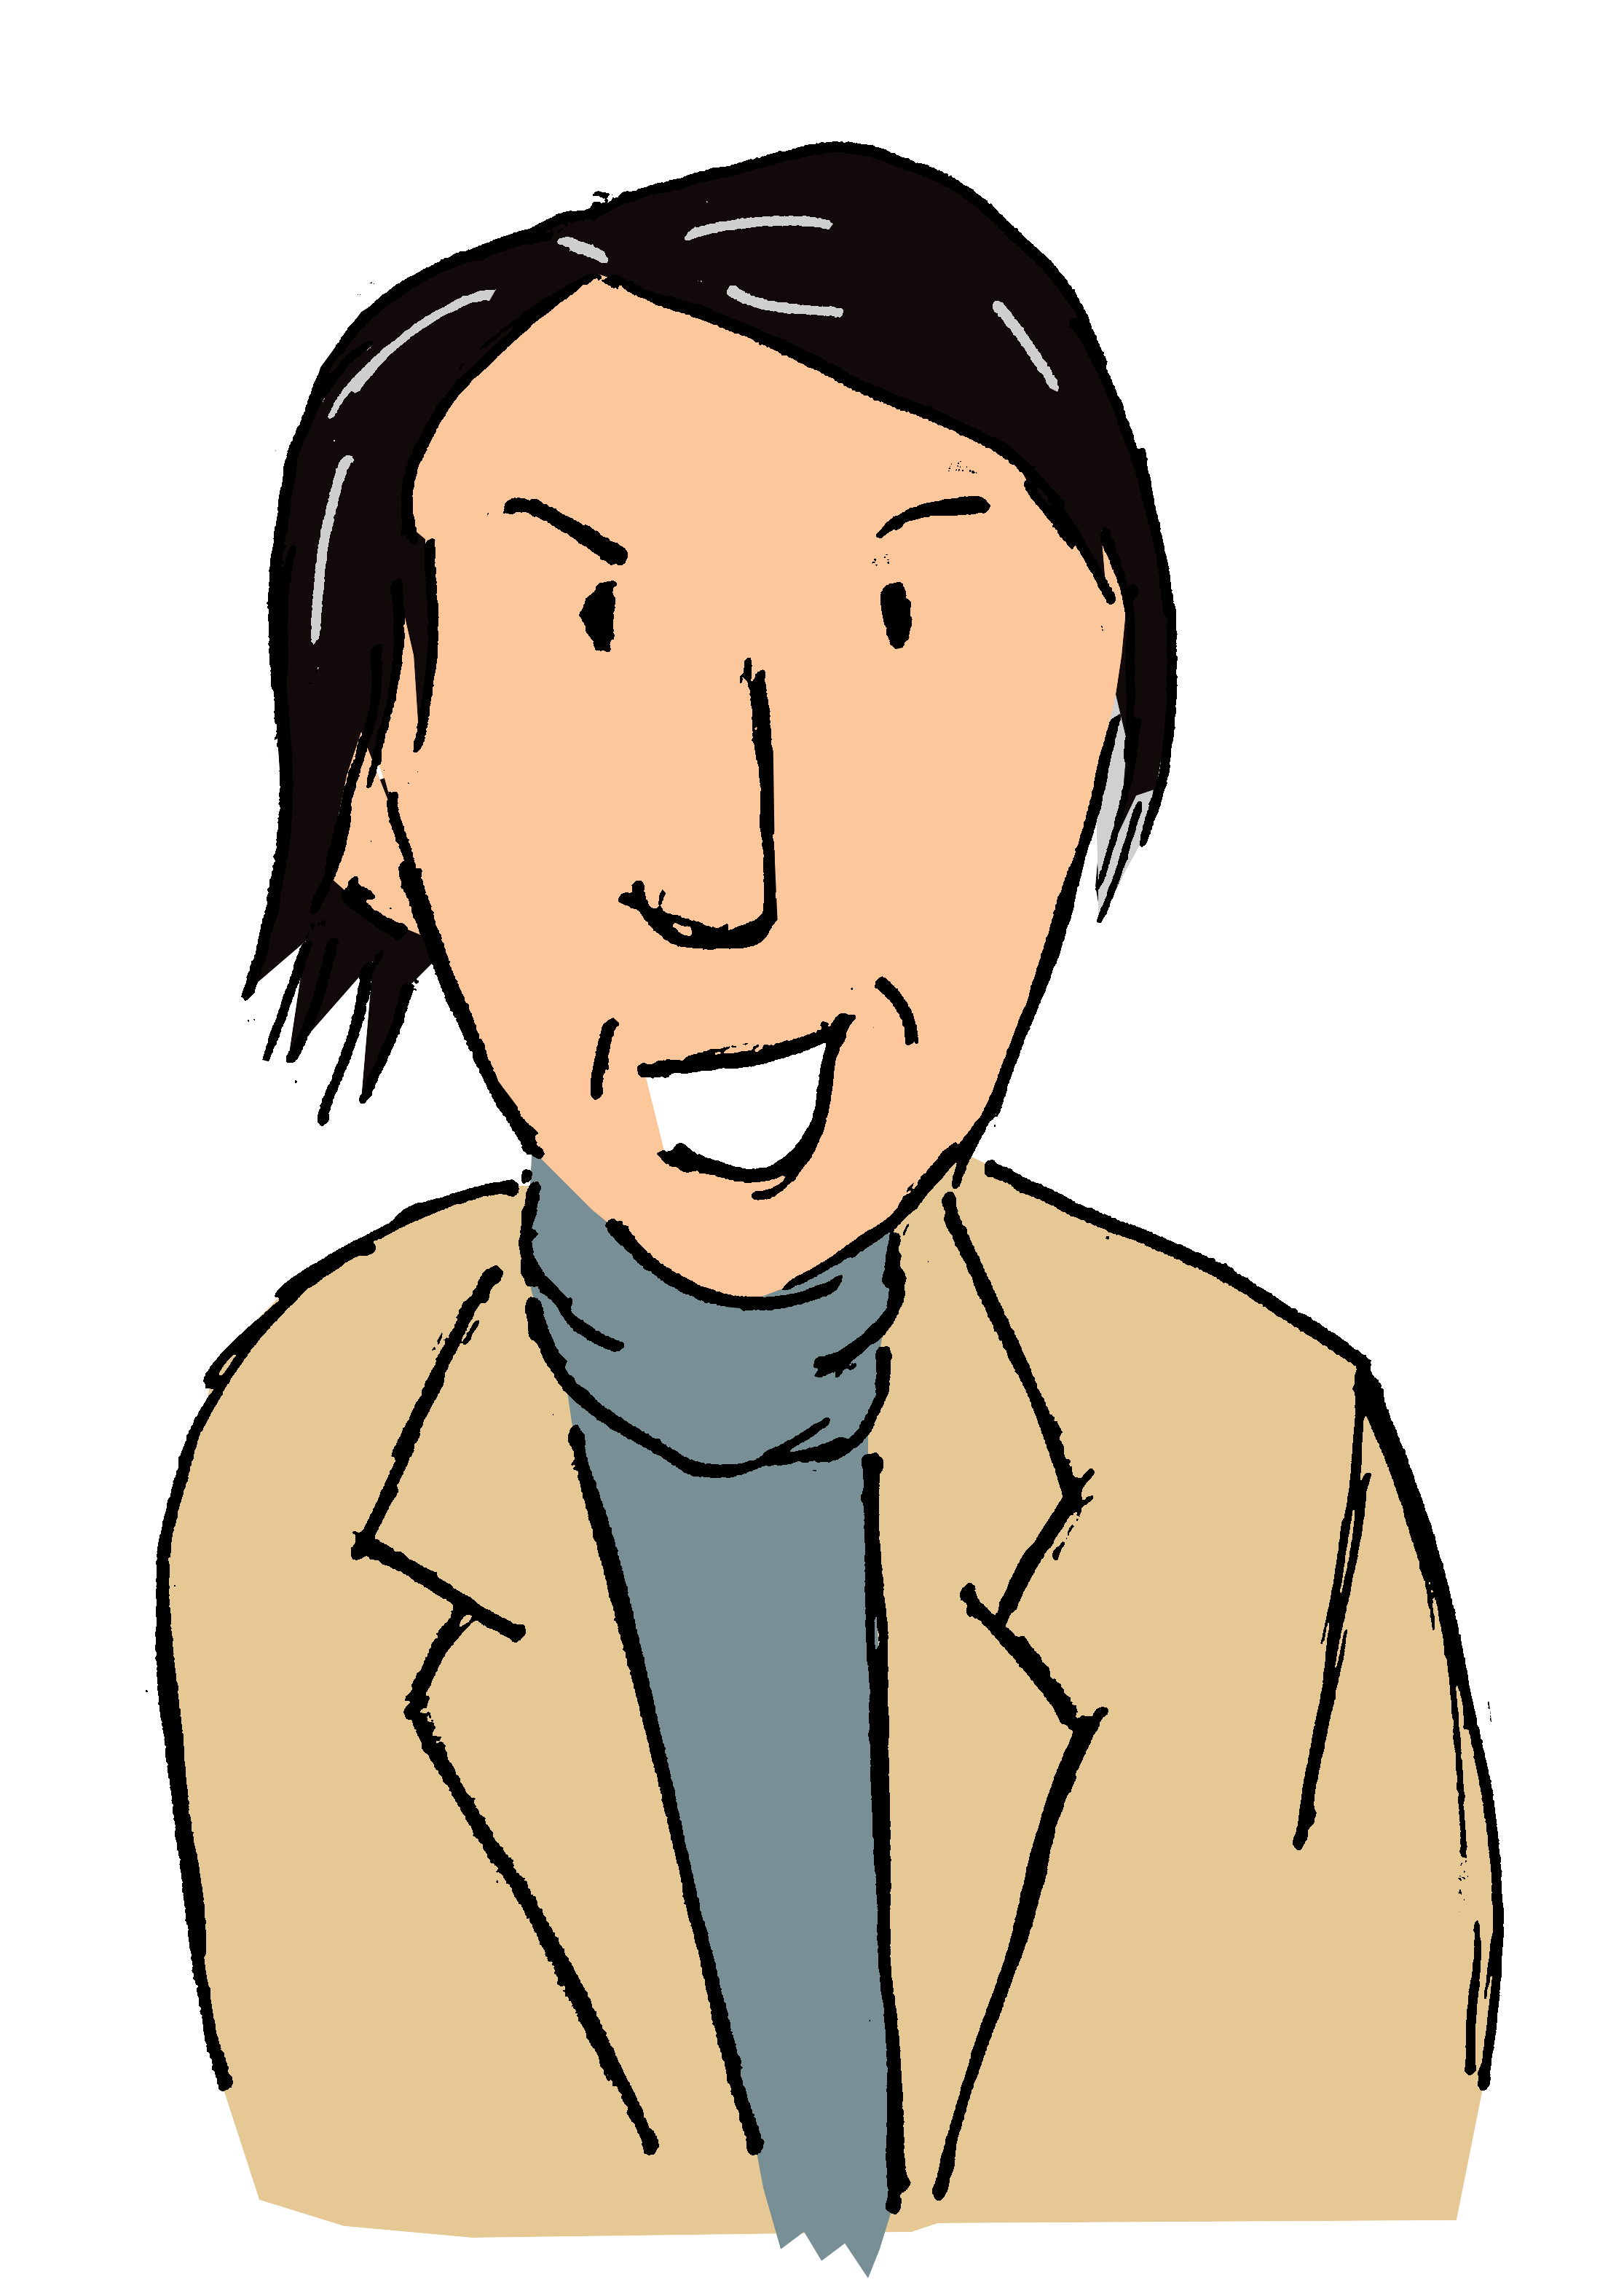
\includegraphics[width=5cm]{carl_sagan}};
			\node (example-textwidth-2) [notice={(-3,0.5)}, ultra thick, right, align=center, text width=12cm, color=black, fill=white, font=\fontsize{23pt}{24pt}\selectfont] at (12,-1) {A bordo delle \emph{Voyager} è stato caricato un disco d'oro contenente una sintesi della cultura umana. Sono stato io stesso, insieme con \textbf{Timothy Ferris}, a supervisionare i contenuti del disco: c'è anche la voce di mio figlio!};
		\end{scope}
		%
		\begin{scope}[shift={(0,-90)}]
			\node at (27,0) () {
\includegraphics[width=3.7cm]{licenza}};
			\node at (18,-0.1) {\textcolor{black}{\fontsize{14}{15}\selectfont Testo e illustrazioni: @ulaulaman - Gianluigi Filippelli}};
		\end{scope}
	\end{tikzpicture}
\end{document}